
%!TeX spellcheck = en-US
%\chapter{Word Embedding and Distributional Features of the web-pages and texts}
\chapter{The Usefulness of Distributed Representations in WGI}

\label{chap:word_embeddings}


%----------------------------------------------------------------------------------------

% Define some commands to keep the formatting separated from the content
\newcommand{\keyword}[1]{\textbf{#1}}
\newcommand{\tabhead}[1]{\textbf{#1}}
\newcommand{\code}[1]{\texttt{#1}}
\newcommand{\file}[1]{\texttt{\bfseries#1}}
\newcommand{\option}[1]{\texttt{\itshape#1}}

%----------------------------------------------------------------------------------------

\section{Introduction}\label{chap:word_embeddings:sec:intro}
 
The most traditional text representation scheme in text mining tasks is the Bag-of-Words (BOW) model which is based on individual tokens as features. It is a simplistic approach to quantify textual information assuming independence of the occurrence of individual tokens in documents. The result is a document vector of high dimensionality (i.e., in the order of thousands of features) and sparseness (i.e., only a few non-zero values per document). The BOW model is not able to capture information about the grammar of documents and completely ignores word order. In addition, it is confused by synonym terms since it assumes they are independent. Nevertheless, it provides an easy and quite competitive approach to represent documents (the W1G scheme used in Chapter \ref{chap:noise} is actually based on BOW).

A more elaborate text representation scheme is to consider n-grams of words (e.g., the W3G model used in Chapter \ref{chap:noise}). This would capture information about word sequences, like phrases. This can improve the ablity of the model to represent syntactic information since the context of words is partially taken into account. Nevertheless, the dimensionality of representation is considerably increased when the order of the model ($n$) is high. In addition, the sparseness of the vectors is increased. It is also possible to apply the n-gram approach on the character level or on POS-tag level, as shown in the experiments of Chapter \ref{chap:noise} (i.e., C4G, POS3G). The main assumption that each feature (n-gram) is independent of the other features is still doubtful in such models.

An alternative approach is to use \textit{distributed representations} that attempt to introduce some kind of dependence of each word (or n-gram) on the other words (or n-grams). For example, the words usually encountered in the context of a specific word are more dependent on that word. In addition, different words found in similar context get a higher share of dependence. Distributed representations can be obtained by applying language modeling methods. Especially, the use of neural network language models and the popular word and document \textit{embeddings} introduced in \parencite{mikolov2013distributed}. 

One main advantage of distributed representations is that they provide compact (i.e., low-dimensional) and dense vectors to quantify syntactic and semantic information in documents. In comparison to regular BOW or n-gram models, distributed features are much less redundant and irrelevant since each such feature captures a combination of information that cannot be specifically determined. Therefore, it seems that open-set WGI methods that are not able to easily handle high-dimensional, sparse vectors with many irrelevant and redundant features would be highly improved by using distributed representations. As already explained in Chapter \ref{chap:openset}, NNDR is an algorithm that, in theory, is vulnerable when it is not combined with appropriate feature sets. The main goal of this Chapter is to examine how the performance of NNDR in WGI tasks is affected when combined with either traditional BOW-like features or distributed features. 

The rest of this chapter is organized as follows. First, the main ideas of distributed representation are presented. Then, the specific distributed features used in this thesis are described. Next, we compare the performance of NNDR using traditional sparse representation schemes with the case dense vectors are used. We also compare these versions of NNDR with OCSVM and RFSE methods and discuss the main conclusions of this study.

\section{Obtaining Distributed Representations}

%The SLM model is defined as the \textit{joint conditional probability distribution} of the next word given the probabilities of previous ones as shown in equation \ref{chap:word_embeddings:eq:slm}

%\begin{equation} \label{chap:word_embeddings:eq:slm}
%	P(w = i) = \prod_{i=1}^{|V|} P(w_{i}|w_{i-k}, ... , w_{i+k})
%\end{equation}
%\noindent
%where $w_{i}$ is the i-th word, and $k$ is for the number of words before or/and and after, writing sub-sequence $w_{i} = (w_{i-k}, w_{i-1}, ... ,w_{i+1}, w_{i+k})$. Note that this model returns a singleton value for a word on the condition of previews or/and next word. This model also can be expanded to have few more words in the conditional probability, usually from 2 up to 4. 

%With this model it can be captured the semantic proximity but it will return zero in the case a sequence have never been met before in the samples. A solution to this problem is the interpolation or smoothness factor that can be applied such as in the \textit{back-off}  model (Katz, 1980 see in bengio2003neural). 

%The model of equation \ref{chap:word_embeddings:eq:slm} can capture the joint probability of word-sequences in terms of feature vectors, however, it cannot capture the correlation of the words in terms of semantics. Models like LSI or LDA are methodologies also been tested in IR and NLP for capturing the semantics in the context of the n-gram based SLM. 

One way to obtain a low-dimensional and dense representation of documents is the use of topic modeling. Topic modeling methods attempt to group terms according to their co-occurrence in documents. They provide a new feature space (composed by latent topics) of pre-defined dimensionality. One popular topic modeling approach is \textit{Latent Semantic Analysis}, a linear algebraic method that transforms a high-dimensional and sparse representation to a low-dimensional and dense one applying \textit{singular value decomposition} \parencite{kontostathis2006framework}. Another popular approach is \textit{Latent Dirichlet Allocation}, a generative probabilistic model where each documents is represented as a mixture over a set of latent topics. Each topic is in turn defined as a distribution over words \parencite{blei2003latent}.

Another main direction that gained huge popularity during the last years is the use of neural probabilistic language models \parencite{bengio2003neural}. We first describe how words can be represented in a continuous space and then we focus on documents.

\subsection{Word Embeddings}

The main idea is that words can be represented by real vectors (word embeddings) that are learned by a neural network \parencite{mikolov2013efficient}. This is unsupervised learning since documents need not be labeled. The neural network is trained to recognize words that occur in similar context. Then, each word is represented in continuous vector space and similar words tend to cluster in the same area. In addition, the distance between related words is affected by semantic similarity (e.g., the difference between terms "king" and "man" is close to the difference between "queen" and "woman") \parencite{mikolov2013efficient}. 

%Then the semantic distance can be approximated by a NNet algorithm given the distribution of the words. The words are initially are having a vector 1-of-V representation, a.k.a. \textit{One-hot representation}. Then the probability of the a word $w_{i}$ in equation \ref{chap:word_embeddings:eq:slm} can be replaced by the real continues vector $t{i}$ and the conditional probability $P(.|.)$ to be approximated my a NNet function $\hat{p}(.)$. The $\hat{}$ (hat) is for symbolizing a special condition where the probability is approximated given a sequence with a specific order, say preceding words or succeeding words or both. 

%Now the DF neural model can be calculated with several architectures where the $\vec{t}$ and the $\hat{p}$ continues distribution can feed separate layers of joint layers, and also the learning strategy can have variant implementations such as Continues Bag-of-Words, Skip-grams etc. The strategy of learning and the NNet architecture are very close related and the results are \textit{continues probability functions with substantially different meaning}, where they can either encode word similarities, word semantics or even paragraph and documents encoding and similarities. 

In practice the distributed features is the mapping of the vocabulary words $V = \{w_{i}, i \in [1, |V|] \}$ to a real vector $\vec{t}_i \in \mathbb{R}^{m}$. One basic architecture is the \textit{Continuous Bag-of-Words} (CBOW) model which attempts to predict a word given its context. This is a \textit{Feedforward Neural Network} with an input layer, a projection layer, and an output layer as shown in figure \ref{chap:word_embeddingss:fig:CBOW_diagram} \parencite{mitra2018introduction}. The input layer is composed by the context of a word (i.e., the few words immediately to its right and left). Every word in the vocabulary is assigned to a \textit{one-hot} vector $t_{i}$ (i.e., a vector of size $|V|$ with all but one values equal to zero). The sequence of context word vectors are added and form the input vector $t_{i*}$. Since the order of words is not important in this setting, the model bears similarities to Bag-of-Words \parencite{mitra2018introduction}.

%W_{in}$ is the weight matrix of the projection layer with regularization parameters $\theta$. Now the $\vec{t}$ is the input to a hidden layer $\vec{h}=\vec{t}H$, which is usually the \textit{hyperbolic tangent hidden layer}, where $H$ is the weights of the hidden layer. Then, the output $\hat{p}=\vec{h}W_{out}$ is the last layer of the NNet.

\begin{figure}[t]
\begin{center}
    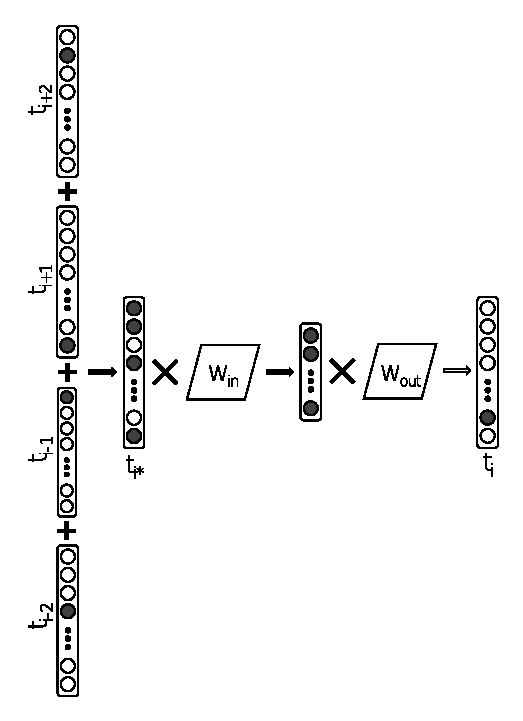
\includegraphics[scale=0.99]{Figures/CBOW_diagram.eps}
	\caption{Architecture of the C-BOW model \parencite{mitra2018introduction}. The network attempts to predict a word given its context words. The order of input words is ignored. The hidden layer has much lower dimensionality in comparison to the one-hot representation of input and output words. The learned weights in $W_{in}$ (and $W_{out}$) can be used as word embeddings.}\label{chap:word_embeddingss:fig:CBOW_diagram}
\end{center}
\end{figure}

%The generic architecture of the final output of the NLM described above is the equation \ref{chap:word_embeddingss:nlm_generic}. Note that the output vector $\vec{y}$ has size $|V|$ due to the input $\hat{w}$ and is the inference model of a \textit{continues distribution} of both the proximity of the words in the sentences (captured by the hidden layer) and the distribution over the vocabulary, which is the continues similarity of the words in this vocabulary. The output layer then is as described in equation \ref{chap:word_embeddings:eq:NLM}

%\begin{equation} \label{chap:word_embeddings:eq:NLM}
%	\vec{y} = \vec{t} + W_{out}(\vec{t}H + b_{h}) + b_{o}
%\end{equation}

%\noindent
%where $b_{o}$ and $b_{h}$ are the output and hidden layers biases. Usually the Hidden layer typically has a size of 500 to 1000 neurons while the projection layer might be 500 to 2000. Due to the multiple layers and the feeding of both the projection and the hidden to the output layer there is great complexity and the process is very computationally demanding. 

%A more efficient method is suggested in \parencite{mikolov2013efficient} where the non-linear hidden layer is removed and the projection layer is shared to all words, geometrically this is equivalent to the projection of the words to the same position. Then the algorithm is reformed and the $\hat{w}$ vectors are replaced by the $t^{*}$ which is the sum of the \textit{one-hot word vectors} \parencite{mitra2018introduction}. 

%Now the equation \ref{chap:word_embeddings:eq:NLM} is becoming \ref{chap:word_embeddings:eq:CBOW}. Due to the new form of the NNet where the tangent hidden layer is absent, there is no constraint in the presenting sequence of the words order. Moreover, the succeeding words also can also be taken in to account in a given \textit{window} say for $k_{w}$ number of words around the specific one. 

The weight matrix $W_{in}$ is of size $|V| \times m$ while $W_{out}$ is of size $m \times |V|$, where $m$ is the size of the hidden layer ($m << |V|$) and it also corresponds to the dimensionality of the extracted distributed representation. The size of the output vector is equal to the vocabulary size. 
%
%\begin{equation} \label{chap:word_embeddings:eq:CBOW}
%	\vec{y} = \hat{t}_{i*} \times W_{out} + b_{o}
%\end{equation}

During training, CBOW attempts to learn weight matrices $W_{in}$ and $W_{out}$. The loss function of CBOW is the following conditional log probability: 

\begin{equation} \label{chap:word_embeddings:eq:CBOW_log_likelihood}
	 \mathcal{L}_{CBOW} = -\frac{1}{|S|} \sum_{i=1}^{|S|}{\log{p(t_{i}|t_{i-k}, ... ,t_{i+k})}}
\end{equation}

\noindent
where $k$ is the size of context words and $S$ is the number of possible context windows in training texts. \textit{Stochastic Gradient Decent} and \textit{Backpropagation} are used to train that network. CBOW is actually an encoder-decoder model and applies a \textit{SoftMax} function in its output:  

\begin{equation} \label{chap:word_embeddings:eq:CBOW_softmax}
	p(t_{i}|t_{i-k},...,t_{i+k}) = \frac{e^{y_{t_{i}}}}{\sum^{|V|}_{i}{e^{y_{t_i}}}}
\end{equation}

\nointdent where $y_{t_i}$ is the output vector for term $t_i$.

Another architecture is the \textit{skip-gram} model, that attempts to predict the context of a word. This is depicted in figure \ref{chap:word_embeddingss:fig:skipgram_diagram} \parencite{mitra2018introduction}. Again, input and output are one-hot vectors while the hidden layer is of dimensionality $m$ ($<<|V|$). The objective is to learn weight matrices $W_{in}$ and $W_{out}$ and the loss function is as follows:

\begin{equation} \label{chap:word_embeddings:eq:skipgram_log_likelihood}
	 \mathcal{L}_{SkipGram} = -\frac{1}{|S|} \sum_{i=1}^{|S|}{ \sum_{-k \leq j \leq +k}{ \log {p(t_{i+j}|t_{i})}  } }
\end{equation}

\noindent where $k$ is the number of context words to be predicted, $S$ the number of all windows in training set, and $p(t_{i+j}|t_{i})$ is obtained as follows:

\begin{equation} \label{chap:word_embeddings:eq:skipgram_softmax}
	p(t_{i+j}|t_{i}) = \frac{ e^{(W_{out}  \times  t_{i+j})^{T} (W_{in} \times  t_{i})}}{\sum^{|V|}_{k=1}{ e^{(W_{out}  \times  t_{k})^{T} (W_{in} \times  t_{i})}}} 
\end{equation}

\begin{figure}[t]
	\begin{center} 
    	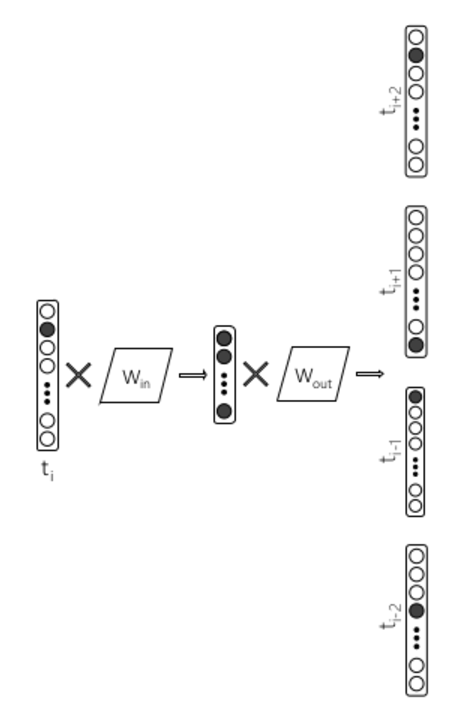
\includegraphics[scale=0.99]{Figures/skip_gram.eps}
		\caption{Architecture of skip-gram model \parencite{mitra2018introduction}. Given a word the network tries to predict its context words. The dimensionality of the hidden layer is much lower than the one-hot representation of input and output words. The learned weights in $W_{in}$ (and $W_{out}$) can be used as word embeddings.}
		\label{chap:word_embeddingss:fig:skipgram_diagram}
	\end{center}
\end{figure}

Finally, the above neural models, either CBOW or skip-grams, since they are approximating the continuous distribution probability function of words over the the Vocabulary $V$ they also satify the following constraint:

\begin{equation} \label{chap:word_embeddings:eq:nnet_condtraint}
	\sum_{i=1}^{|V|}{p(t_{i}|t_{i-k}, ... ,t_{i+k})} = 1
\end{equation}

Note that in both CBOW and skip-gram models the two weight matrices $W_{in}$ and $W_{out}$ can be used to provide the word embeddings\footnote{An implementation of these methods is provided in https://github.com/tmikolov/word2vec}. Usually $W_{in}$ plays this role and $W_{out}$ is discarded.

%\textcolor{red}{THIS IS NOT CLEAR: A very important difference between the CBOW and skip-grams is the NNet architecture usually their implementation is based. Particularly, there are some internal detail occurring because of the objective of the task. \parencite{boden2002guide}}

To summarize, the above models are very effective \textit{Language Modeling} approaches having the ability to quantify simultaneously syntanctic and semantic information of words. They provide a \textit{distributed representation} for words (i.e., each word is represented with a dense vector which is a point in a space of relatively low dimensionality). However, it is not easy to understand the actual meaning of each dimension in this space. The sequence of words in texts is now considered and can also be applied in cases input texts are composed of sequences of characters or POS tags.

Finally, the training of the CBOW and the skip-gram models can be expensive despite the fact of limiting the number of hidden layers. However, there are several engineering solution that are accelerating the training time, such as \textit{Huffman binary tree encoding} of words and \textit{hierarchical softmax}. The latter is a solution that enables us to use multi-processing power and update the weight parameters concurrently. The parallel asynchronous updating of the parameter matrices is not conforming to the mathematical constraints however in practice the negative effect is minor. Huffman binary tree is a method for compressing the encoding of terms where the ones with the higher frequency are accessed faster. In addition to this, \textit{negative sampling}, \textit{sub-sampling}, or \textit{ramdom sampling} are also used where in the range of $k$ window for surrounding words only a few ones are selected during training with minor effect in  performance and significant acceleration in training \parencite{mikolov2013efficient,mitra2018introduction}.  

\subsection{Document Embeddings} \label{chap:word_embeddings:sec:PVBOW} 
 
There are several approaches to transform word embeddings to document embeddings \parencite{mitra2018introduction,mikolov2013distributed}. The most simple method produces a vector for a given document by averaging the word embeddings of the words in a document. It is also possible to modify the network architecture and work on the sentence level. For example, word embeddings per sentence are averaged and the goal is to predict a sentence given its context sentences \parencite{kenter2016}. Another idea, the \textit{Sent2Vec} method~\footnote{An implementation of this method can be found in https://github.com/epfml/sent2vec}, is to compose sentence embeddings by extending CBOW to include word vectors and word n-gram embeddings \parencite{pagliardini-etal-2018-unsupervised}.

In this thesis, we use the \textit{Doc2Vec} approach, introduced in \parencite{le2014distributed}, that attempts to generalize the word embeddings methods to work with sequences of words. The main idea is to train a neural network so that to learn embeddings for entire documents (or passages). There are two versions of this approach that are analogous to CBOW and skip-gram models. 

%\usepackage{authblk}

The \textit{Paragraph Vector - Distributed Memory} (PV-DV) model is based on CBOW. The task is to train a network to predict the next word in a text window given the paragraph vector and the word vectors of its context (actually the preceding words). The paragraph (it could be entire document) vector is considered as memory of the words distribution and aims to capture general information like the topic of the document. 

Another approach, following the skip-grams paradigm, is to ignore the context words in the input, and train a model for predicting a context word given its paragraph vector. This method, called \textit{Paragraph Vector - Distributed Bag-of-Words} (PV-DBOW), is depicted in figure \ref{chap:word_embeddingss:fig:PVBOW_diagram}. In practice, at each iteration of stochastic gradient descent, a text window of size $k$ is sampled. Then, a random word is sampled from the text window and form a classification task given the paragraph vector. This model requires to store less data, because only the SoftMax weights are stored as opposed to both SoftMax weights and word vectors in the PV-DM. 

The loss function of PV-DBOW (a modification of the corresponding skip-gram loss function shown in formula \ref{chap:word_embeddings:eq:skipgram_log_likelihood} is as follows: 

\begin{equation} \label{chap:word_embeddings:eq:pvbow_log_likelihood}
	 \mathcal{L}_{SkipGram} = -\frac{1}{|S|} \sum_{i=1}^{|S|}{ \sum_{-k \leq j \leq +k}{ \log {p(t_{i+j}|D_{i})}  } }
\end{equation}
\noindent
where $D_{i}$ is the document vector of $i$-th document, $S$ is the number of windows over the training texts and $k$ is the number of words to be predicted surrounding the input word. Consequently,  the SoftMax function for the output of the model is modified as follows:

\begin{equation} \label{chap:word_embeddings:eq:pvbow_softmax}
	p(t_{i+j}|t_{i}) = \frac{ e^{(W_{out}  \times  t_{i+j})^{T} (W_{in} \times  D_{i})}}{\sum^{|V|}_{i}{ e^{(W_{out}  \times  t_{k})^{T} (W_{in} \times  D_{i})}}} 
\end{equation}

\begin{figure}[t]
\begin{center} 
    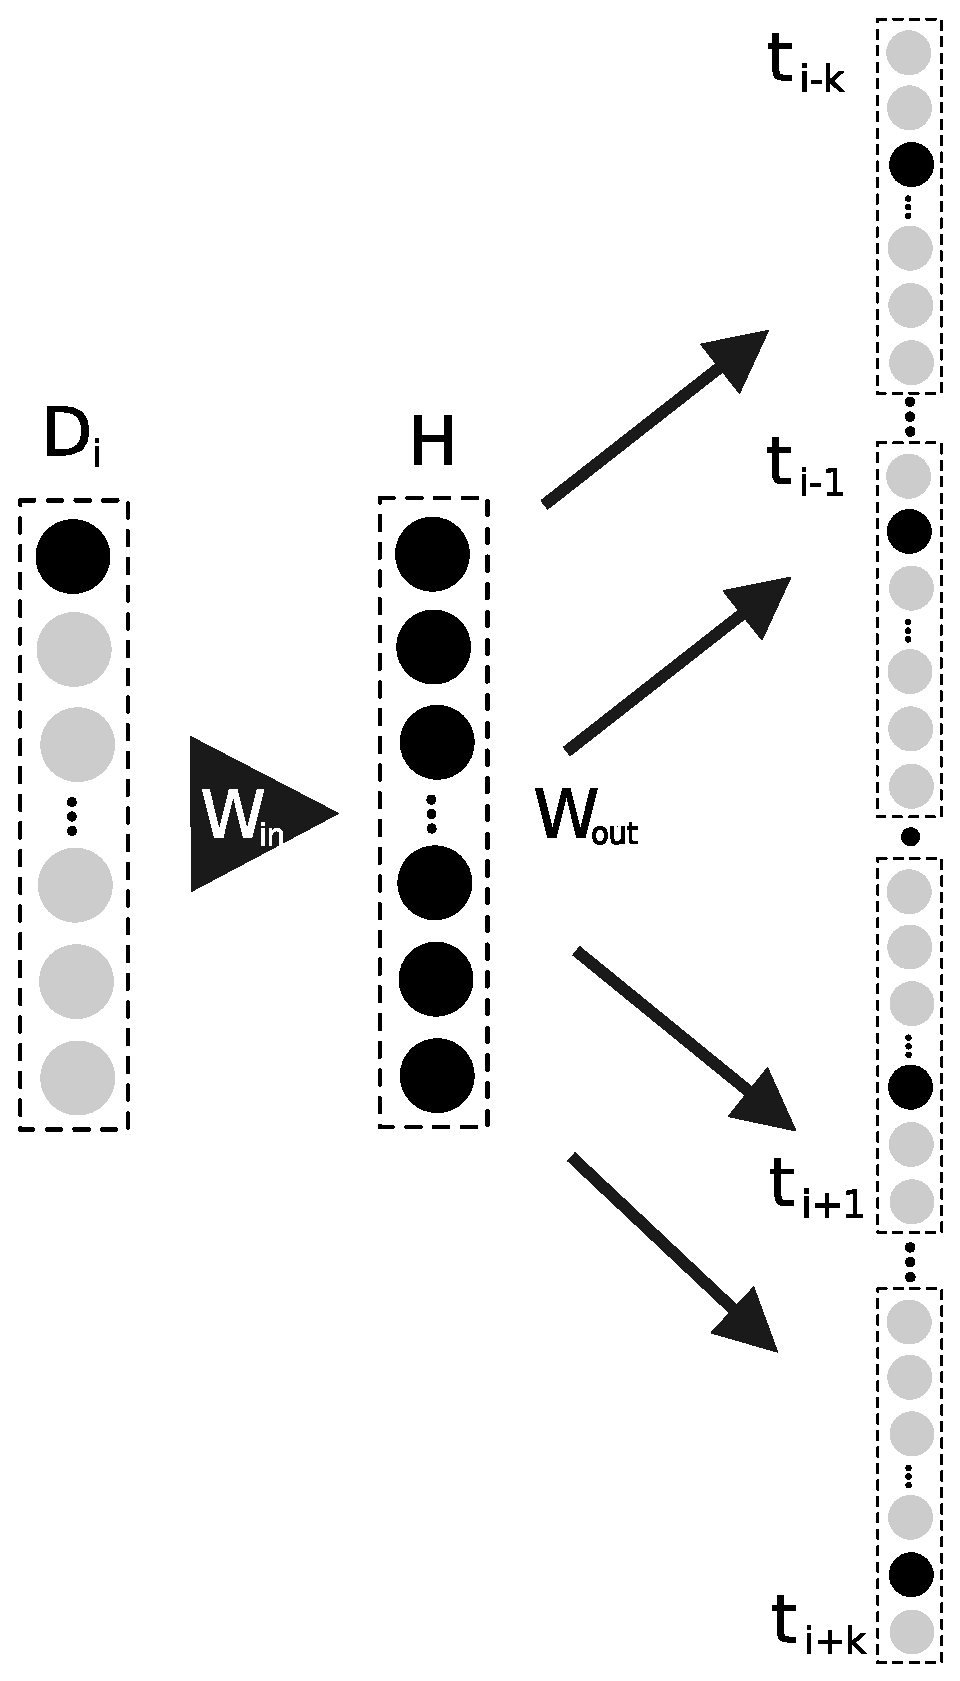
\includegraphics[scale=0.50]{Figures/pvbow.eps}
    \caption{Architecture of PV-DBOW. Given a paragraph vector, predict context words.}
	\label{chap:word_embeddingss:fig:PVBOW_diagram}
\end{center}
\end{figure}

There are several modifications for the PV-DBOW method aiming to increase its efficiency including, \textit{document frequency based negative sampling} and \textit{document length regularization} \parencite{le2014distributed,posadas2017application}. It should be noted that the paragraph vectors could be used to represent  sentences, paragraphs, or entire documents. In this study, the whole web-page is considered. In addition the input texts could be sequences of characters, POS tags, character n-grams, word n-grams etc.

This method of producing document embeddings has successfully been used in several text classification tasks \parencite{le2014distributed}. Its main advantage over traditional BOW and n-gram representation schemes is that it provides compact and dense vectors that include a rich combination of syntactic semantic and stylistic information of documents.

\section{Experimental Setup}\label{chap:word_embeddings:sec:experiments_setup}

In this chapter, the usefulness of the previously described distributed representation of documents is examined in the framework of open-set WGI. As already explained, NNDR is vulnerable when combined with a text representation scheme of irrelevant and redundant features. In this thesis, NNDR is used in combination with \textit{Distributed Features} (DF), obtained by the PV-DBOW approach. We compare this new method with NNDR using traditional BOW and n-gram features as well as with other open-set methods (OCSVM and RFSE).

%\subsection{Corpus}\label{chap:word_embeddings:sec:experiments_corpora}

The experiments of this chapter are based on \textit{SANTINIS}, a benchmark corpus, as described in Chapter \ref{chap:noise}. Briefly, this dataset comprises 1,400 English web-pages evenly distributed into seven genres (blog, eshop, FAQ, frontpage, listing, personal home page, search page) as well as 80 BBC web-pages evenly categorized into four additional genres (DIY mini-guide, editorial, features, short-bio). In addition, the dataset comprises a random selection of 1,000 English web-pages taken from the SPIRIT corpus \parencite{joho2004spirit}. The latter can be viewed as \textit{unstructured noise} since genre labels are missing.

The PV-DBOW models have been trained using the whole corpus. Note that the training of this approach is unsupervised (i.e., the genre labels are not taken into account). The corpus initially is split to a set of paragraphs, as required from PV-DBOW. To be more specific, the paragraphs are sentences split from all the documents of the whole corpus. We examine three different variations, using either sequences of word unigrams (W1G), word trigrams (W3G) or character 4-grams (C4G) as input texts (W1G correspond to texts in their original form). Each type of n-grams is used separately as suggested in \parencite{posadas2017application}. The dimensionality of document embeddings is selected from $DF_{dim}=\{50,100,250,500,1000\}$. 

In addition, the terms with very low-frequency in the training set are discarded. In this study, we examine $f_{min}=\{3,10\}$ as frequency cutoff threshold. The text window size is selected from $W_{size}=\{3,8,20\}$. The remaining parameters of PV-DBOW are set as follows: $\alpha=0.025$, $epochs=\{1, 3, 10\}$ and $decay=\{0.002, 0.02\}$. 

In practice, a library for HTML removal and and vector representation of the web-pages has been created for this work, named  \textit{Html2Vec}\footnote{\url{https://github.com/dpritsos/html2vec}}. There is a special module for PV-DBOW modeling that has been built based on the the implementation of the algorithm found in \textit{Gensim} package \footnote{\url{https://github.com/RaRe-Technologies/gensim}}. 

We also represent documents with traditional representation schemes to conduct comparative experiments. Similar to PV-DBOW, we extract regular C4G, W1G, and W3G. For each of these schemes, we use Term-Frequency weights (we use TF to refer to this kind of traditional feature as opposed to DF for distributed features). The feature space for TF is defined by a vocabulary $V_{TF}$, which is extracted based on the most frequent terms of the training set. We consider $V_{TF}=\{5k,10k,50k,100k\}$. 

Regarding the NNRD open-set classifier, there are two parameters, $lambda$ and DRT, and their considered values are: $\lambda =\{0.2, 0.5, 0.7\}$, $DRT\textit{=\{0.4, 0.6, 0.8, 0.9\}}$, $p_{1} = \{0.5, 0.7\}$, $p_{2} = \{03, 0.5\}$. All aforementioned parameters are adjusted based on grid-search using only the training part of the corpus.

The parameter tuning for OCSVM and RFSE methods has been performed as described in Chapter \ref{chap:noise} for the SANTINIS corpus. The reported evaluation results are obtained by performing 10-fold cross-validation and, in each fold, the full set of 1,000 noise pages is included. This evaluation strategy is giving a more realistic evaluation. Since the noise size is greater than the size of any known genre.

To compensate the unbalanced distribution of web pages over the genres because of the noise part, the open-set macro-averaged precision, recall, and $F_{1}$ measures are used \parencite{mendesjunior2016}. Note again than this variant of evaluation measures ignores the unknown class.  

Finally, for selecting the parameter settings that obtain optimal evaluation performance, two scalar measures are used: the Area under the macro Precision-Recall Curve (AUC) of 11 standard Recall levels and the macro-averaged $F_{1}$ ($F_1^{macro}$) score.

\section{Experimental Results}\label{chap:word_embeddings:sec:results}

\subsection{The Effect of Distributed Representation on NNDR}\label{chap:word_embeddings:sec:NNDR_PVBOW_vs_BOW}

Initially NNDR is evaluated using the traditional TF scheme as shown in Table \ref{chap:word_embeddings:tbl:NNDR_TF}. The overall performance is poor. NNDR seems to work better with W3G features. Note that the dimensionality of this representation is quite high. The performance of the algorithm is slightly affected by parameter tuning for splitting ratios $p_{1}$ and $p_{2}$ while DRT in all cases is $0.8$. The method seems to be robust to the examined values of $\lambda$ regularization parameter. It should also be noted that both $F_1$ and AUC are maximized for the same parameter settings and document representation.

\begin{table}[t]
\center
\begin{tabular}{cccccccccc}
\hline
$p_{1}$ & $p_{2}$ & DRT & $\lambda$ & Features & Dim. & $P_{macro}$ & R_{macro} & $AUC_{macro}$ & $F_1^{macro}$ \\
\hline
0.7 & 0.3 & 0.8 & any & C4G & 5000 & 0.664 & 0.403 & 0.291 & 0.502 \\
0.7 & 0.5 & 0.8 & any & W1G & 5000 & 0.691 & 0.439 & 0.348 & 0.537 \\
0.5 & 0.5 & 0.8 & any & W3G & 10000 & \textbf{0.720} & \textbf{0.664} & \textbf{0.486} & \textbf{0.691} \\
\hline
\end{tabular}
\caption{Maximum performance of NNDR with traditional (TF) Features on SANTINIS coprus. $p_{1}$ and $p_{2}$ are the splitting ratios to form simulated noise and DRT is the threshold. $\lambda$ is the regulation parameter used in the normalized accuracy. Dim. is the dimensionality of representation. The evaluation measures are the open-set variants of macro-averaged precision, recall, $F_1$, and AUC of the precision-recall curve.}
\label{chap:word_embeddings:tbl:NNDR_TF}
\end{table}

\begin{table}
\center
\begin{tabular}{cccccccccc}
\hline
$p_{1}$ & $p_{2}$ & DRT & $\lambda$ & Features & Dim. & $P_{macro}$ & R_{macro} & $AUC_{macro}$ & $F_1^{macro}$ \\
\hline
any & any & 0.8 & any & C4G & 50 & \textbf{0.829} & 0.600 & 0.455 & 0.696 \\
any & any & 0.8 & any & W1G & 50 & 0.733 & \textbf{0.670} & 0.541 & 0.700 \\
any & any & 0.8 & any & W3G & 100 & 0.827 & 0.615 & \textbf{0.564} & \textbf{0.706} \\
\hline
\end{tabular}
\caption {Maximum performance of NNDR with distributed features on SANTINIS coprus. $p_{1}$ and $p_{2}$ are the splitting ratios to form simulated noise and DRT is the threshold. $\lambda$ is the regulation parameter used in the normalized accuracy. Dim. is the dimensionality of representation. The evaluation measures are the open-set variants of macro-averaged precision, recall, $F_1$, and AUC of the precision-recall curve.}
\label{chap:word_embeddings:tbl:NNDR_PVBOW}
\end{table}

The evaluation of NNDR combined with PV-DBOW features is shown in Table \ref{chap:word_embeddings:tbl:NNDR_PVBOW}. As can be seen, in two out of three types of features (C4G and W1G) the performance of the algorithm is significantly improved in terms of both macro $F_{1}$ and AUC. The best overall performance is still acquired by W3G features and it is slightly improved in comparison to the respective results when TF representation is used (the improvement is considerably higher for AUC measure). DF seems to particularly enhance precision results for C4G features and recall results for W1G features. 

These results are obtained using a much lower dimensionality of representation (i.e., an order of magnitude lower than TF scheme). This demonstrates that NNDR is better able to cope with the compactness and density of DF vectors. It should also be noted that the robustness of the model is increased since the best results are acquired for exactly the same parameter settings and most NNDR parameters do not affect the obtained performance. 

A more detailed view of the performance of NNDR when combined with either traditional or distributed W3G features is depicted in PRCs of Figure  \ref{chap:word_embeddings:fig:NNDR_W3G}. Note that in both cases the same parameter settings are used for the NNDR classifier.  As can be seen, the precision of the model based on DF remains high for more standard recall levels in comparison to TF which is significantly affected by the presence of noise. This means that DF is particularly useful in WGI applications where precision is considered more important than recall. The two approaches have comparable performance when recall reaches 0.5 although DF still outperforms TF. The points where curves stop indicate the percentage of the corpus that has been classified as unknown which is similar in both cases (i.e., about 40\% of the corpus).

\begin{figure}[t]

\begin{center}
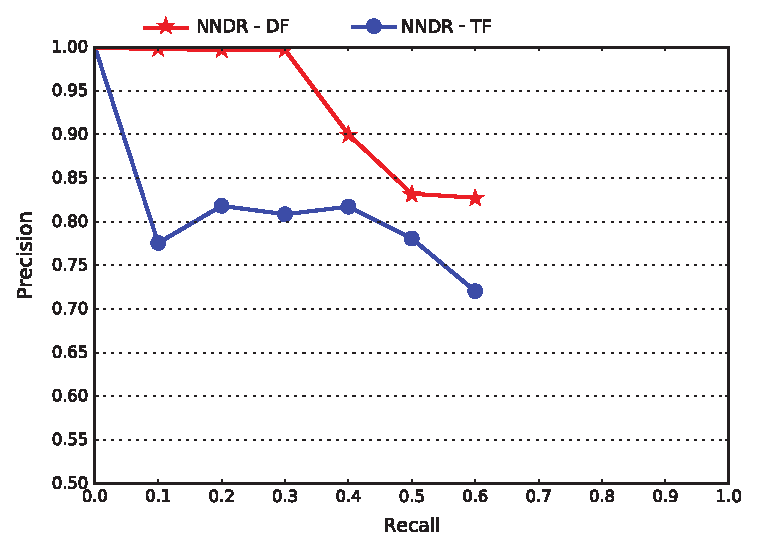
\includegraphics[scale=0.99]{Figures/NNDR_W3G.eps}
\caption{Precision-Recall curves of NNDR on SANTINIS corpus for traditional (TF) and distributed (DF) W3G features.}
\label{chap:word_embeddings:fig:NNDR_W3G}
\end{center}

\end{figure}

\subsection{Comparison of Open-set WGI Methods}\label{chap:word_embeddings:sec:experiments_setup}

In this section, the performance of NNDR on the SANTINIS corpus is compared to that of OCSVM and RFSE obtained as described in Chapter \ref{chap:noise}. The experimental setup for NNDR with either TF or DF schemes is exactly the same therefore the evaluation results for these models are directly comparable. In the framework of this experiment, OCSVM and RFSE serve as baseline models to help us see how competitive the NNDR approach can be when it is assisted by DF representation in unstructured noise conditions.

\begin{table}[t]
\center
\caption {Performance of baselines and NNDR on the SANTINIS coprus. All evaluation scores are macro-averaged.}
\label{chap:word_embeddings:tbl:NNDR_RFSE_OCSVME_final}
\begin{tabular}{ccccccc}
\hline
Model & Features & Dim. & Precision & Recall & AUC & F1 \\
\hline
RFSE & TF-C4G & 50k & 0.739 & \textbf{0.780} & 0.652 & 0.759 \\
RFSE & TF-W1G & 50k & 0.776 & 0.758 & \textbf{0.657} & \textbf{0.767} \\
RFSE & TF-W3G & 50k & 0.797 & 0.722 & 0.615 & 0.758 \\
OCSVM & TF-C4G & 5k & 0.662 & 0.367 & 0.210 & 0.472\\
OCSVM & TF-W1G & 5k & 0.332 & 0.344 & 0.150 & 0.338\\
OCSVM & TF-W3G & 10k & 0.631 & 0.654 & 0.536 & 0.643\\
NNDR & TF-C4G & 5k & 0.664 & 0.403 & 0.291 & 0.502 \\
NNDR & TF-W1G & 5k & 0.691 & 0.439 & 0.348 & 0.537 \\
NNDR & TF-W3G & 10k & 0.720 & 0.664 & 0.486 & 0.691 \\
NNDR & DF-C4G & 50 & \textbf{0.829} & 0.600 & 0.455 & 0.696 \\
NNDR & DF-W1G & 50 & 0.733 & 0.670 & 0.541 & 0.700 \\
NNDR & DF-W3G & 100 & 0.827 & 0.615 & 0.564 & 0.706 \\
\hline
\end{tabular}
\end{table}

First, NNDR with TF features is compared with the baselines. In this case, NNDR outperforms OCSVM. On the other hand, RFSE performed NNDR in both macro-averaged $F_{1}$ and AUC. This is consistent for any kind of features (C4G, W1G, or W3G). The RFSE model is the top overall performer while both OCSVM and NNDR are significantly low in respect of AUC, $F_{1}$ and precision. Only, NNDR with TF scheme for W3G is competitive. 

There is notable difference in the dimensionality of representation used by the examined approaches though. RFSE relies upon a 50k-manifold while NNDR and OCSVM are based on much lower dimensional spaces. This demonstrates the ability of RFSE to exploit the existence of redundant feature sets. It has to be noted that RFSE builds an ensemble by iteratively and randomly selecting a subset of the available features. That way, it internally reduces the dimensionality for each constituent base classifier (RFSE is using 1,000 randomly selected features from the 50,000 most frequent features in each repetition). 

Next, NNDR with DF is compared with the same baselines. Although there is a notable improvement for NNDR using DF, it is still outperformed by RFSE in terms of both $F_{1}$ and AUC. On the other hand, NNDR returns a notably higher performance than RFSE with respect to precision for C4G and W3G features. This indicates that NNDR using DF could be more useful than RFSE in WGI applications where precision is more important than recall.

A closer look at  the comparison of the examined methods is provided in Fig. \ref{chap:word_embeddings:fig:NNDR_W3G_Best_RFSE_Baseline}, where macro-averaged precision-recall curves are depicted. The NNDR-DF model maintains very high precision scores for low levels of recall. Particularly, for W3G features the difference between NNDR-DF and RFSE at that point is clearer. NNDR-TF is clearly worse than both NNDR-DF and RFSE. In addition, OCSVM is competitive in terms of precision only when W3G features are used but its performance drops abruptly in comparison to that of NNDR-DF. 

RFSE with W1G performs significantly better in terms of precision than NNDR (with DF). It also manages to recognize correctly larger part of the corpus, more than $70\%$ either for W3G or for W1G, as compared to NNDR-DF that reaches $60\%$ in both cases. 

\begin{figure}[t]
\begin{center}
    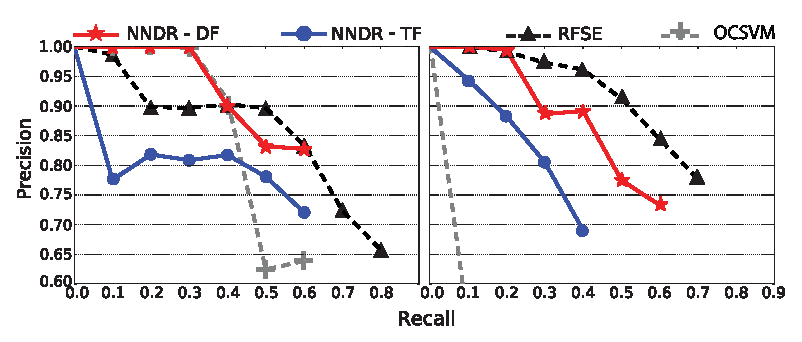
\includegraphics[scale=0.95]{Figures/NNDR_W3G-W1G_Best_RFSE-OCSVM-Baselines.eps}
	\caption{Precision curves in 11-standard recall levels of the examined open-set classifiers using either W3G features (left) or W1G features (right).}
	\label{chap:word_embeddings:fig:NNDR_W3G_Best_RFSE_Baseline}
	\end{center}
\end{figure}

%, i.e. the remaining part after the last mark of each curve it the percentage of the corpus tha has been classified as Unknown from the algorithms.

\section{Conclusions}\label{chap:word_embeddings:sec:conclusions}

In this chapter, we presented an experimental study focused on WGI and the use of distributed features in combination with an open-set classifier that obtained promising results in other domains \parencite{mendesjunior2016}. Our experiments are based on a benchmark corpus with unstructured noise already used in previous work and a strong baseline. 

It seems that distributional features provide a significant enhancement to the performance of NNDR in WGI tasks. The low-dimensionality and density of DF are crucial to enhance the performance of NNDR which suffers from the presence of irrelevant and redundant features (as any nearest-neighbor method). Yet, RFSE proves to be a hard-to-beat baseline at the expense of relying upon a much higher representation space (usually in the thousands of features). However, with respect to precision, NNDR with PV-DBOW features is much more conservative and it prefers to leave web-pages unclassified rather than predicting an inaccurate genre label. Depending on the application of WGI, precision can be considered much more important than recall and this is where the proposed approach seems more suitable (e.g., web-page ranking applications).

Further research could focus on more appropriate distance measures within NNDR specially with recent data-driven features obtained with powerful NLP convolutional and recurrent deep networks. Moreover, alternative types of distributed features could be used (e.g., topic modeling or pre-trained language models). Finally, a combination of NNDR with RFSE models could be studied as they seem to exploit complementary views of the same problem.

